\chapter{High-Rate Data Acquisition Pipeline} \label{ch:Pipeline}

Before anything else, I would like to clarify that this project is exclusively dedicated to studying the Data Link layer and the Physical layer according to the \textsf{OSI} model.

There are different strategies for structuring reliable communication. The \(\mathsf{CHESS}\) \(\mathsf{Pathfinder\text{-}0}\) communication architecture strictly adheres to the standards \href{https://ccsds.org/publications/}{\texttt{CCSDS publications}} developed by the \(\mathsf{Consultative}\) \(\mathsf{Committee}\) \(\mathsf{for}\) \(\mathsf{Space}\) \(\mathsf{Data}\) \(\mathsf{Systems}\) (CCSDS). The physical layer is governed by \autocite{CCSDS_401_0_B_32}, which defines \(\mathsf{X\text{-}Band}\) modulation parameters, while \autocite{CCSDS_131_0_B_5} and \autocite{CCSDS_132_0_B_3} dictate the synchronization markers, \(\mathsf{FEC}\) schemes such as \(\mathsf{Reed\text{-}Solomon}\) and \(\mathsf{Viterbi}\), and the data link protocols essential for space-grade framing. The mentioned documents are the \(\mathcal{B}lue\) \(\mathcal{B}ooks\). Theoretical rationale is derived from the \(\mathcal{G}reen\) \(\mathcal{B}ooks\) \autocite{CCSDS_130_1_G_3}, with operational best practices and administrative procedures guided by the \(\mathcal{M}agenta\) and \(\mathcal{S}ilver\) series, respectively.

Although the ultimate goal of this project is to deploy a receiver, a complete transmitter pipeline was also implemented to generate valid test signals, simulate the transmission channel, and plot the necessary performance metrics.

\section{TM Synchronization and Channel Coding} \label{sec:tm_sync_coding}

Following the CCSDS standard, in the synchronization and channel coding sublayer ($\mathcal{B}lue$ $\mathcal{B}ook$ \autocite{CCSDS_131_0_B_5}), we must implement the blocks shown in \Cref{fig:diagram1_tx} and \Cref{fig:diagram1_rx}. A concatenated coding configuration has been chosen, with Reed-Solomon as the outer code and a convolutional coder as the inner code. This is because it offers the highest code gain, and we will see in \Cref{ch:Link} why it is the only viable combination.

% Transmitter Diagram
\begin{figure}[!ht]
    \centering
    
\includegraphics[width=0.9\textwidth]{diagram1tx.pdf}
    \caption{Block diagram of the transmitter.}
    \label{fig:diagram1_tx}
\end{figure}

The concatenated configuration of Reed-Solomon (RS) and convolutional code (CC) provides a robust system with manageable decoding complexity. In this architecture, the inner convolutional code (typically processed by a Viterbi decoder) is responsible for correcting most of the channel errors, such as thermal noise (AWGN). However, by design, the Viterbi decoding process characteristically outputs residual errors in concentrated bursts.

% Receiver Diagram
\begin{figure}[!ht]
    \centering
    
\includegraphics[width=0.9\textwidth]{diagram1rx.pdf}
    \caption{Block diagram of the receiver.}
    \label{fig:diagram1_rx}
\end{figure}

This is where the outer Reed-Solomon code acts as the perfect complement to mitigate these bursts. Since the RS decoder processes information by symbols, the fact that residual Viterbi errors arrive clustered is highly advantageous: multiple erroneous bits concentrated in a single symbol count as just one symbol error for the RS code. Thus, the combination of both codes efficiently corrects both AWGN and burst errors without overwhelming the system's capacity.


\section{Reed Solomon Coding} \label{sec:rs}

As introduced in \Cref{sec:tm_sync_coding}, the Reed-Solomon ($\mathsf{RS}$) code acts as the outer error-correcting mechanism in the $\mathsf{CCSDS}$ telemetry architecture \autocite{CCSDS_131_0_B_5}. While the inner Viterbi decoder efficiently processes additive white Gaussian noise ($\mathsf{AWGN}$), as we mentioned, it characteristically outputs residual errors in concentrated bursts when metric crossovers occur (see \Cref{fig:frame_plot}). $\mathsf{RS}$ codes are non-binary cyclic block codes optimally suited to mitigate this exact phenomenon, as their error-correction capability is independent of the number of bit errors contained within a single corrupted symbol.

\subsection{Mathematical Characterization}

The $\mathsf{CCSDS}$ standard specifies a systematic $\mathsf{RS}$ code defined over the Galois field $\mathbb{F}_{2^8}$ (or $\mathsf{GF}(2^8)$). The fundamental building block is the $J$-bit symbol, where $J=8$, resulting in an alphabet size of $2^8 = 256$ discrete elements \autocite[Section 5.1]{CCSDS_130_1_G_3}. The block length $n$ of the codeword in symbols is dictated by the relationship $n = 2^J - 1$, yielding a standard unshortened length of $n = 255$ symbols.

To achieve maximum performance, the standard defines an information block size $k = 223$ symbols. The code's minimum distance $d_{min}$ determines its error-correcting bounds:
\begin{equation}
    d_{min} = n - k + 1 = 255 - 223 + 1 = 33
\end{equation}
From this distance metric, the maximum number of correctable symbol errors $E$ per codeword is mathematically guaranteed as:
\begin{equation}
    E = \left\lfloor \frac{d_{min} - 1}{2} \right\rfloor = 16
\end{equation}
Consequently, the systematic encoder appends $2E = 32$ parity check symbols to the original $223$ information symbols, forming a total transmitted codeword of $2040$ bits.

\begin{figure}[!ht]
    \centering
    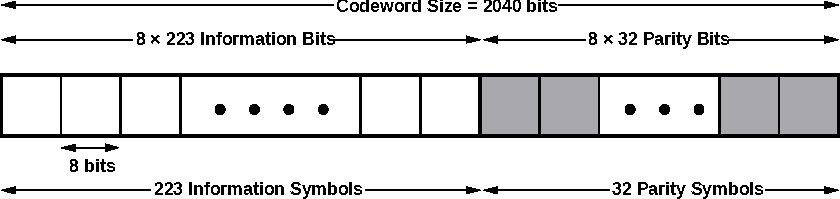
\includegraphics[width=0.75\textwidth]{figures/Inkscape/RS_codeword.pdf} 
    \caption{Structure of the systematic $\mathsf{CCSDS}$ (255, 223) Reed-Solomon codeword, illustrating the payload and appended parity symbols.}
    \label{fig:rs_codeword}
\end{figure}

\subsection{Field and Code Generator Polynomials}

The arithmetic operations governing the encoding process require a strictly defined finite field. The $\mathsf{CCSDS}$ standard constructs $\mathbb{F}_{2^8}$ using the following primitive field generator polynomial over $\mathbb{F}_{2}$:
\begin{equation}
    F(x) = x^8 + x^7 + x^2 + x + 1
\end{equation}
Let $\alpha$ be a root of $F(x)$ such that $F(\alpha) = 0$. The specific code generator polynomial $\bm{g}(x)$ over $\mathbb{F}_{2^8}$, which dictates the mapping of the systematic parity symbols, is constructed as a self-reciprocal polynomial (palindrome) to minimize hardware multiplier complexity \autocite[Section 5.2]{CCSDS_130_1_G_3}:
\begin{equation}
    g(x) = \prod_{j=128-E}^{127+E}(x-\alpha^{11j}) = \sum_{i=0}^{2E} G_{i} x^{i}
\end{equation}
Furthermore, the standard mandates a $\mathsf{Dual}$ $\mathsf{Basis}$ symbol representation for transmission \autocite[Section 4.3.9]{CCSDS_131_0_B_5}. Instead of the conventional polynomial basis $(1, \alpha^1, \dots, \alpha^7)$, the symbols are transformed into a dual basis defined by the trace function $Tr(z)$. This specific algebraic mapping ensures standardized hardware compatibility across different mission architectures.

\subsection{Symbol Interleaving}

As previously established, the Viterbi decoder produces error bursts that can easily exceed the $E=16$ symbol correction limit of a single $\mathsf{RS}$ codeword. To preserve the $\mathsf{FEC}$ integrity, the standard employs rectangular block interleaving with a depth $I \in \{1, 2, 3, 4, 5, 8\}$ \autocite[Section 4.3.5]{CCSDS_131_0_B_5}.

The interleaving process is mathematically equivalent to writing $I$ consecutive $\mathsf{RS}$ codewords into an $I \times n$ matrix. The symbols are written row-by-row but transmitted column-by-column. 

\begin{figure}[!ht]
    \centering
    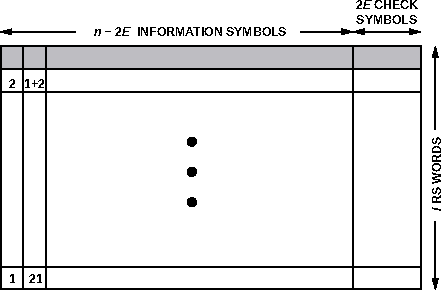
\includegraphics[width=0.5\textwidth]{figures/Inkscape/RS_interleaver.pdf} 
    \caption{Rectangular block interleaver matrix of depth $I$. A contiguous channel error burst of length $\mathcal{B}$ symbols is distributed upon de-interleaving such that no single codeword absorbs more than $\lceil \mathcal{B}/I \rceil$ errors. You can find an example in \Cref{fig:interleaver_example}.}
    \label{fig:rs_interleaver}
\end{figure}

Upon reception, the de-interleaver performs the inverse transposition. By spreading a contiguous burst of $\mathcal{B}$ channel errors across $I$ distinct codewords, the effective number of errors per codeword is reduced to approximately $\mathcal{B}/I$. As long as the degraded symbols per row remain $\leq E$, the Reed-Solomon algebraic decoder can successfully reconstruct the original transmitted frame without data loss.


\section{Convolutional Coding} \label{sec:cc}

The convolutional coding scheme established for space telemetry \autocite[Section 3]{CCSDS_131_0_B_5} is defined as a linear mapping over the Galois field $\mathbb{F}_{2}$. This specific implementation is a non-systematic, transparent code with a constraint length $K=7$ and a fundamental code rate $r=1/2$, \Cref{fig:cc_diagram}. The mathematical structure of the encoder is best described in the transform domain using the delay operator $D$, where the input sequence $\bm{u}(D)$ is transformed into an output codeword $\bm{v}(D)$ through the generator matrix $\bm{G}(D) = [G_{1}(D), G_{2}(D)]$.

The generator polynomials, expressed in their octal representation as $171_{8}$ and $133_{8}$, are defined by the following structural equations:
\begin{align*}
    G_{1}(D) &= 1 + D + D^{2} + D^{3} + D^{6} \\
    G_{2}(D) &= 1 + D^{2} + D^{3} + D^{5} + D^{6}
\end{align*}
The encoding process is mathematically defined as the discrete convolution of the input sequence $\bm{u} \in \mathbb{F}_{2}^{\infty}$ with the impulse responses $\bm{g}_{i}$ of the generator polynomials, where for each information bit $u_{k}$ at time $k$, the encoder generates a raw symbol pair $(c_{1,k}, c_{2,k})$ according to the linear mapping \begin{equation}
    c_{i,k} = \sum_{j=0}^{K-1} u_{k-j} \cdot g_{i,j} \\\textcolor{gray}{\pmod 2}.
\end{equation} While these generator outputs $\bm{c}_{i}(D) = \bm{u}(D)G_{i}(D)$ establish the error-correcting structure, the standard mandates a non-linear $\mathsf{Inversion}$ transformation specifically on the second stream to guarantee a high Transition Density within the channel. Consequently, the final transmitted symbols $v_{k,1}$ and $v_{k,2}$ are formulated as $v_{k,1} = c_{1,k}$ and $v_{k,2} = c_{2,k} \oplus 1$, a structural modification that ensures the sequence $\bm{v}$ remains alternating even during periods of null input data ($u_{k}=0$), thereby providing the receiver's symbol synchronizer with the necessary edges to maintain a stable lock in the extremely low \(\mathsf{SNR}\) conditions characteristic of deep space missions.
\begin{figure}[h]
    \centering
    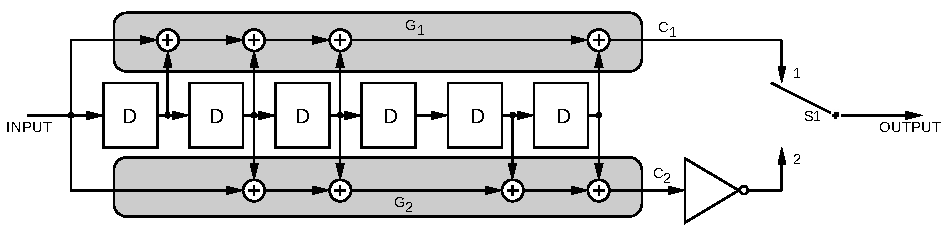
\includegraphics[width=0.8\textwidth]{figures/Inkscape/cc_diagram.pdf} 
    \caption{The CCSDS Standard Convolutional Code: Constraint Length K=7, Rate 1/2.}
    \label{fig:cc_diagram} 
\end{figure}

The code $\mathcal{C}$ is inherently transparent, a property defined as $\mathsf{f}(\overline{\bm{u}}) = \overline{\mathsf{f}(\bm{u})}$. This characteristic allows the $\mathpzc{Viterbi}$ decoder to resolve the $180^{\circ}$ phase ambiguity inherent in BPSK and QPSK modulations. If the demodulator captures the signal with inverted polarity, the decoder produces the inverted version of the original data, which can then be corrected by the frame layer without losing the coding gain.

\subsection{Distance Metrics and Performance Characteristics}

The error-correcting capability of the code is determined by its minimum free distance, $d_{free}$, which represents the minimum Hamming distance between any two distinct infinite-length paths in the $\mathpzc{trellis}$ diagram. For the $K=7$ code, the $d_{free}$ is exactly $10$\footnote{Exhaustive searches for rate $1/2$ codes confirm that $d_{free}=10$ is the absolute mathematical maximum achievable for a constraint length $K=7$. This specific code was selected as a local optimum because it maximizes error-correcting performance while remaining within the $2^{K-1}=64$ state computational limit of the Viterbi decoders available during its standardization. You can find more information here \autocite[Section 4.2]{CCSDS_130_1_G_3}.}. From this metric, we derive the maximum number of symbol errors $t$ that the decoder is guaranteed to correct within a specific observation window:
\begin{equation}
    t = \left\lfloor \frac{d_{free} - 1}{2} \right\rfloor = \left\lfloor \frac{10 - 1}{2} \right\rfloor = 4
\end{equation}
In the presence of additive white Gaussian noise (AWGN), the asymptotic coding gain is proportional to $r  d_{free}$. For this $r=1/2$ code, the distance properties provide a significant reduction in the required $E_{b}/N_{0}$ to achieve a target bit error rate, typically yielding a gain of approximately $5.5$ dB at a BER of $10^{-5}$ when compared to uncoded BPSK.

\subsection{Punctured Architectures for Spectral Efficiency}

When bandwidth constraints require a higher spectral efficiency $\eta$ than what the $r=1/2$ code provides, the standard employs a puncturing operator $\mathsf{P}_{\mu}$ \autocite[Section 4.3]{CCSDS_130_1_G_3}. This process involves the systematic deletion of symbols from the output of the rate $1/2$ encoder according to a puncturing pattern $\bm{m}$, enabling alternative code rates such as $r \in \{2/3, 3/4, 5/6, 7/8\}$. However, a rate of 1/2 is chosen to improve signal integrity. 
\begin{comment}
While puncturing increases the effective data rate, it results in a reduction of the effective free distance $d_{free, p}$ of the code. The choice of the rate $r$ is therefore a critical design trade-off between the available transmitter power and the allocated frequency bandwidth. It is also noted that the convolutional decoder may produce error bursts; therefore, the standard recommends the use of an outer $\mathsf{Frame\_Check}$ sequence or a cyclic redundancy check (CRC) to validate the integrity of the $\mathpzc{decoded}$ frames before they are passed to the $\mathbb{D}$ata $\mathbb{L}$ink $\mathbb{P}$rotocol sublayer.
\end{comment}

\subsection{Optimal Detection} \label{subsec:detection}
The optimal detection of convolutional codes is mathematically formulated as a $\mathsf{Maximum}$ $\mathsf{Likelihood}$ sequence estimation problem where the objective is to minimize the probability of word error by selecting the most probable path through the $\mathpzc{trellis}$, see \Cref{fig:trellis_diagram}. Given a received sequence $\bm{Z}$, the decoder identifies the message $\bm{U}^{(m')}$ that maximizes the conditional probability density function, or likelihood function, which is formally expressed as:
\begin{equation}
    P(\bm{Z}|\bm{U}^{(m')}) = \max_{\text{all } \bm{U}^{(m)}} P(\bm{Z}|\bm{U}^{(m)})
\end{equation}
In the presence of additive white Gaussian noise ($\mathsf{AWGN}$), maximizing this likelihood is equivalent to minimizing the cumulative squared Euclidean distance between the received symbols $z_{ji}$ and the candidate codeword symbols $v_{ji}^{(m)}$. The total path metric $\mathcal{M}$ for a sequence of length $\mathcal{L}$ symbols is computed as follows:
\begin{equation}
    \mathcal{M} = \sum_{j=1}^{\mathcal{L}} \sum_{i=1}^{n} (z_{ji} - v_{ji}^{(m)})^2
\end{equation}
This global optimization is efficiently executed by the $\mathtt{Viterbi}$ algorithm, which decomposes the problem into a recursive series of local decisions based on the state transitions of the encoder.

\begin{figure}[h]
    \centering
    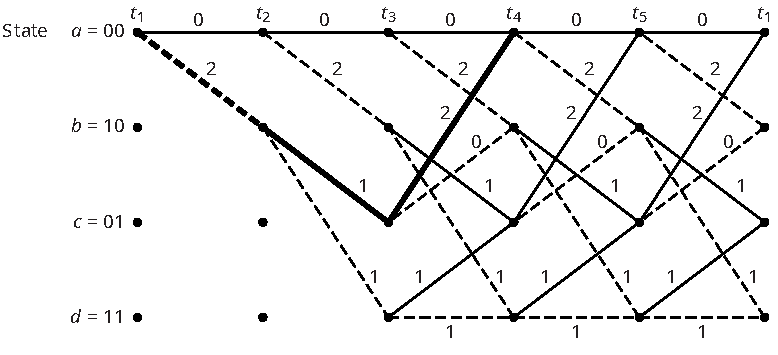
\includegraphics[width=0.7\textwidth]{figures/Inkscape/trellis.pdf} 
    \caption{Example of Trellis diagram \autocite[Figure 7.7]{Sklar2001}, labeled with distances from the all-zeros path. K=3.}
    \label{fig:trellis_diagram} 
\end{figure}

A significant characteristic of the $\mathtt{Viterbi}$ decoding process is the nature of its residual errors, which typically appear as error bursts rather than independent bit errors. These bursts occur when the channel noise is sufficient to cause a metric crossover, forcing the decoder to deviate from the correct path and follow an incorrect branch until the cumulative metrics allow the paths to re-merge. Because these error bursts are statistically correlated and span several constraint lengths, they can significantly degrade the performance of subsequent protocols that assume independent error distributions. This necessitates the use of a $\mathsf{Frame\:Error\:Control\:Field}$ ($\mathtt{FECF}$) based on a cyclic redundancy check ($\mathtt{CRC}$) or the concatenation with an outer block code like Reed-Solomon to ensure the integrity of the decoded data frames.

\begin{figure}[h]
    \centering
    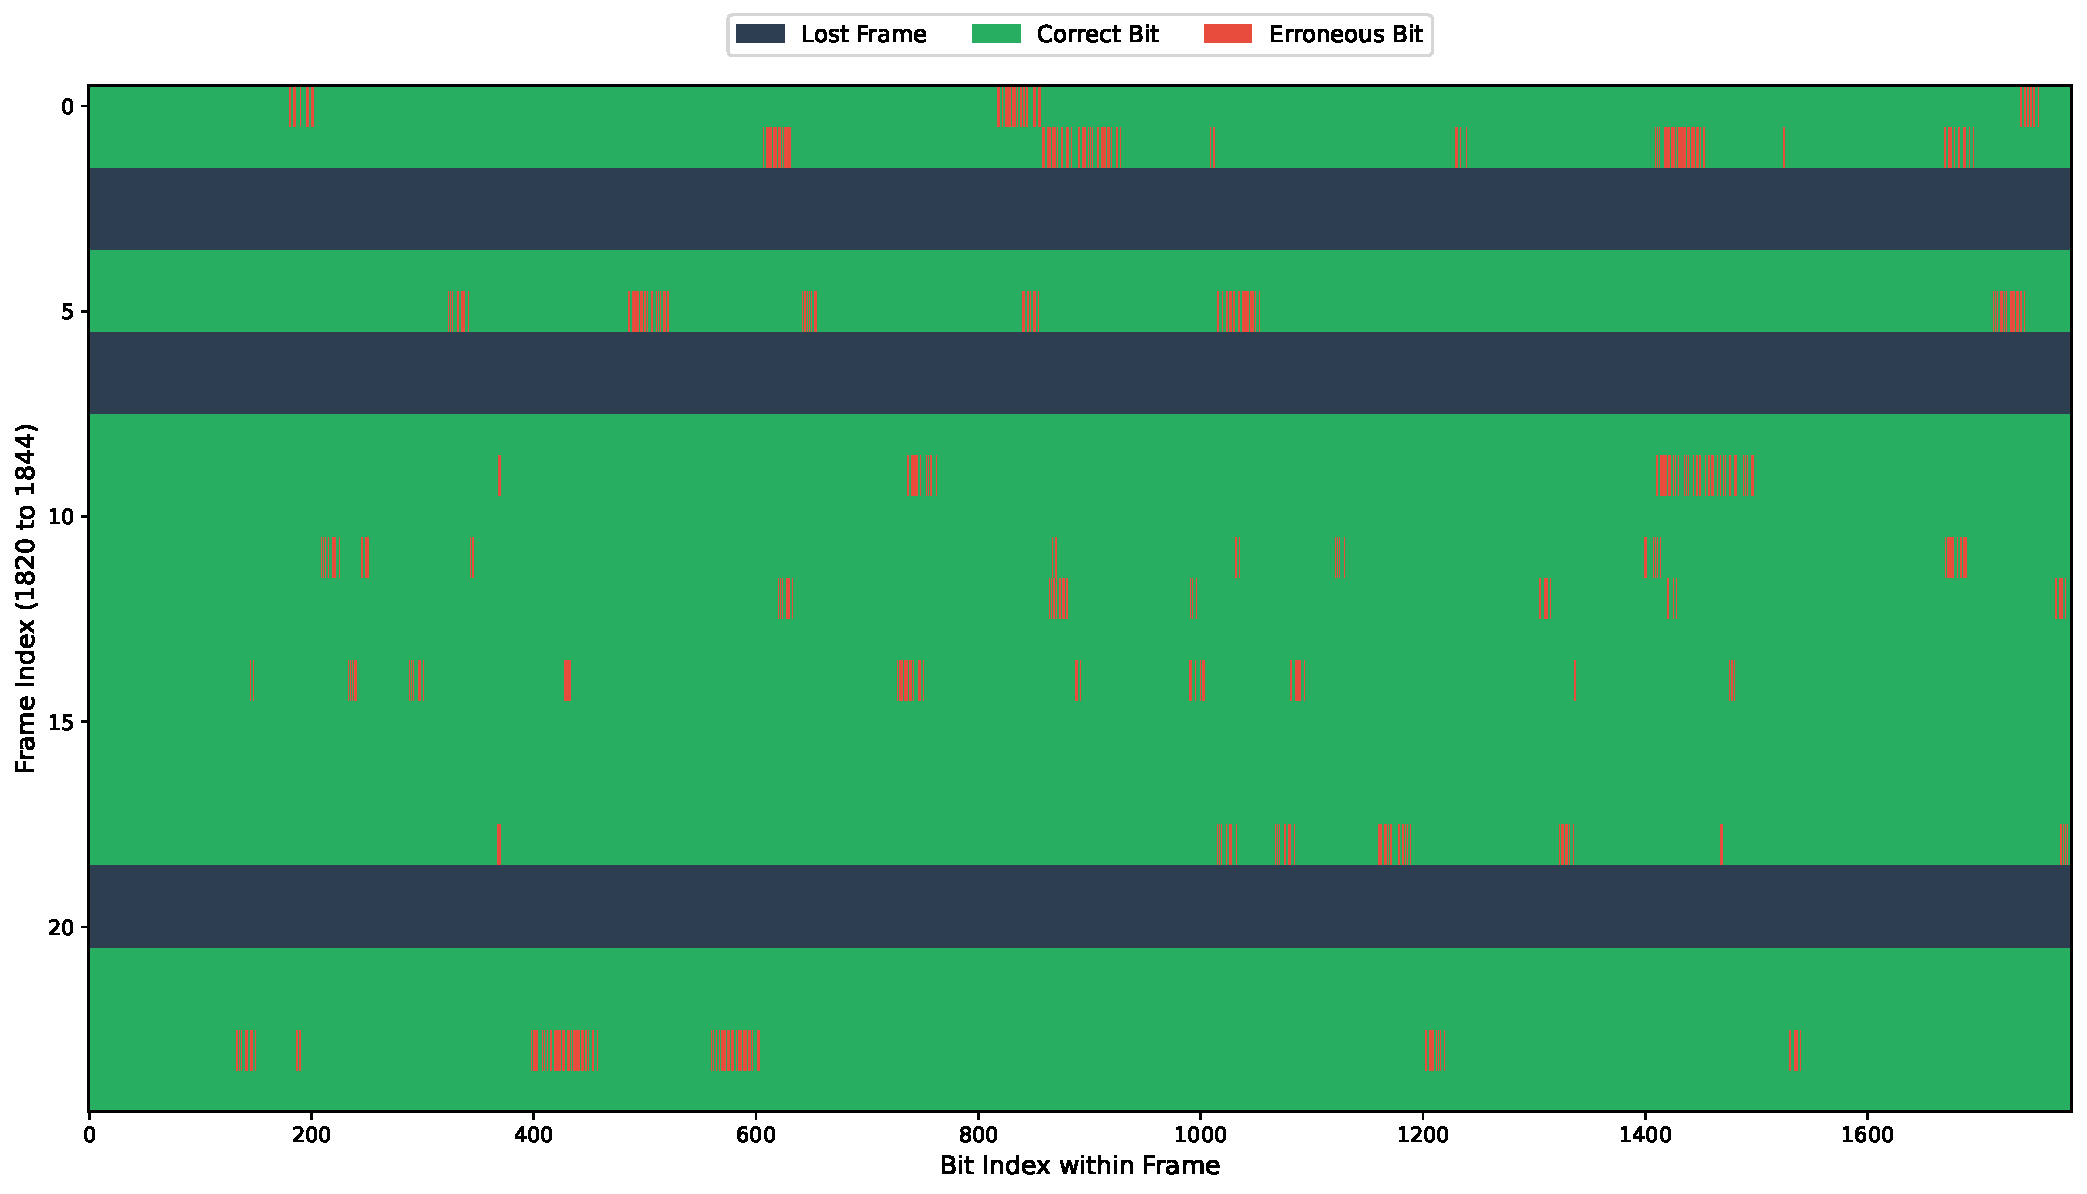
\includegraphics[width=1\textwidth]{figures/Inkscape/frame_plot.pdf} 
    \caption{2D Map: Bit Errors and ASM Loss when $E_b/N_0 = 3.8$ dB.}
    \label{fig:frame_plot} 
\end{figure}

In \Cref{fig:frame_plot}, you can see an example of what happens at low $\mathsf{SNR}$. The plot shows different frames (in rows) found by the synchronization algorithm after the $\mathtt{Viterbi}$ decoder. You can see how errors (in red) mostly occur in bursts; that’s when the decoder takes the wrong path and takes a few bits to get back on track. When these error bursts hit the ASM frame, they destroy it, making it hard to recover the frame and leading to those gray gaps in the image.

% Already in RS so not important here
%Subsequently\todo[author=Daniel]{This can be moved to section Reed Solomon}, the $\mathpzc{Reed}\text{-}\mathpzc{Solomon}$ code will be able to correct a finite number of errors. You can observe that some frames are error-free while others contain many. By using an interleaver with the appropriate depth, we can significantly reduce the $\mathsf{BER}$, as shown in \autocite[Figure 6-10]{CCSDS_130_1_G_3}.


\section{Data Randomization (Pseudo-randomizer)} \label{sec:pr}

Despite the excellent error-correcting properties of the analyzed codes, these linear schemes cannot guarantee on their own a sufficient number of bit transitions in the communication channel. The presence of prolonged sequences of constant bits (such as contiguous bursts of zeros or ones) critically degrades the performance of clock recovery devices at the receiver, causing symbol synchronizers to lose phase lock. To ensure a high bit transition density, mitigate the formation of discrete spectral lines in the radiated signal, and facilitate rapid carrier acquisition, the $\mathsf{CCSDS}$ standard mandates the application of a pseudo-randomization block ($\mathsf{Pseudo\text{-}randomizer}$) to the data sequence prior to transmission.

The implementation of this subsystem is conventionally structured using an $8$-stage linear feedback shift register $\mathtt{LFSR}$, governed by the irreducible generator polynomial $h(x) = x^8 + x^7 + x^5 + x^3 + 1$ over the Galois field $\mathbb{F}_{2}$. This circuit generates a deterministic pseudo-random sequence with a maximum period of $255$ bits that is combined with the structured codeblock via a bit-by-bit $\mathtt{XOR}$ operation. Due to the symmetric nature of this algebraic transformation, the process is completely reversible at the receiving end. 

\section{Physical Layer Architecture} \label{sec:physical_layer}


The physical layer is responsible for the continuous-time representation of the discrete symbol stream, translating logical states into propagating electromagnetic waveforms. In adherence to the stringent spectral occupancy regulations defined by the \textsf{CCSDS} for X-Band communications \autocite{CCSDS_401_0_B_32}, the communication architecture relies on a Quadrature Phase Shift Keying (QPSK) modulation scheme, strictly governed by band-limiting pulse shaping techniques. This section delineates the mathematical models and digital signal processing blocks implemented within the continuous-time baseband architecture.

\subsection{Modulation and Spectral Containment}

To mitigate adjacent channel interference and satisfy the maximum bandwidth constraints without introducing Inter-Symbol Interference (ISI), the system employs a Square Root Raised Cosine (SRRC) filter \autocite{Artes2007}. The CCSDS Blue Book \autocite[Section 2.4.18]{CCSDS_401_0_B_32} enforces the use of SRRC filtering to achieve optimal spectral containment for high-rate data transmissions. Let $T_s$ denote the channel symbol duration. The frequency response of the SRRC filter, $H(f)$, is mathematically parameterized by the roll-off factor $\alpha$, and is formulated as:
\begin{equation}
H(f) = \begin{cases}
1, & |f| < \frac{1-\alpha}{2T_s} \\
\sqrt{\frac{1}{2} \left[ 1 + \sin\left(\frac{\pi T_s}{\alpha} \left( \frac{1}{2T_s} - |f| \right) \right) \right]}, & \frac{1-\alpha}{2T_s} \le |f| \le \frac{1+\alpha}{2T_s} \\
0, & |f| > \frac{1+\alpha}{2T_s}
\end{cases}
\end{equation}
In this specific implementation, the roll-off factor is established at $\alpha = 0.5$ (\texttt{excess\_bw = 0.5}), meticulously balancing the trade-off between spectral efficiency and timing jitter immunity. The digital QPSK modulator maps the coded data into complex baseband symbols $s_k \in \{\pm 1 \pm j\}$, which are subsequently up-sampled by a factor of $SPS = 2$ and convolved with the discrete-time SRRC impulse response. 

\subsection{Synchronization and Carrier Recovery}

Following the optimal minimum-distance detector rationale \autocite{Proakis2007}, the receiver must flawlessly estimate both the symbol timing and the residual carrier phase to accurately project the received vector onto the QPSK decision regions. To resolve the fractional delay embedded in the asynchronous sampling process, a Polyphase Filter Bank (PFB) clock synchronizer is utilized. This algorithm employs a Maximum Likelihood derivative matched filter to track the timing error, continuously adjusting the decimated sample selection through a closed-loop interpolator \autocite{Artes2007}.

Once the optimal symbol epochs are recovered, the residual phase offsets and subtle frequency drifts are tracked utilizing a Costas loop configured for fourth-order symmetry. This is detailed in \Cref{ch:Doppler}.




